\documentclass[aspectratio=169,11pt]{beamer}
% =====================================================================
%  pds-beamer.tex — Estilo común de las transparencias.
%
%  Uso (desde teoría/Tx/transparencias/):
%     \documentclass[aspectratio=169,11pt]{beamer}
%     % =====================================================================
%  pds-beamer.tex — Estilo común de las transparencias.
%
%  Uso (desde teoría/Tx/transparencias/):
%     \documentclass[aspectratio=169,11pt]{beamer}
%     % =====================================================================
%  pds-beamer.tex — Estilo común de las transparencias.
%
%  Uso (desde teoría/Tx/transparencias/):
%     \documentclass[aspectratio=169,11pt]{beamer}
%     \input{../../comun/pds-beamer}
%     \title{...}  \subtitle{Tema x · ...}
%     \begin{document}
%       \portada
%       ...
%     \end{document}
%  Compilar con:  latexmk -xelatex  (o «make» desde teoría/)
% =====================================================================

\usetheme{Boadilla}
\usecolortheme{orchid}
\usefonttheme{professionalfonts}
\setbeamercovered{transparent}
\setbeamersize{text margin left=0.8cm, text margin right=0.8cm}
\setbeamertemplate{navigation symbols}{}
\setbeamertemplate{itemize item}[square]
\setbeamertemplate{itemize subitem}[circle]
\setbeamertemplate{itemize subsubitem}[triangle]
\setbeamertemplate{enumerate item}[square]
\setbeamertemplate{enumerate subitem}[circle]
\setbeamertemplate{caption}{\raggedright\insertcaption\par}

\input{../../comun/pds-comun.tex}

% Tipografía: Fira Sans + Fira Math (legibles en proyector)
\usepackage{fontspec}
\usepackage{unicode-math}
% Se cargan por nombre de fichero para que funcionen con cualquier
% instalación de TeX Live (o MiKTeX) sin instalar fuentes en el sistema.
\setmainfont{FiraSans}[Extension=.otf, UprightFont=*-Regular, BoldFont=*-SemiBold,
  ItalicFont=*-Italic, BoldItalicFont=*-SemiBoldItalic]
\setsansfont{FiraSans}[Extension=.otf, UprightFont=*-Regular, BoldFont=*-SemiBold,
  ItalicFont=*-Italic, BoldItalicFont=*-SemiBoldItalic]
\setmonofont{FiraMono}[Extension=.otf, UprightFont=*-Regular, BoldFont=*-Medium, AutoFakeSlant=0.15, Scale=0.92]
\setmathfont{FiraMath-Regular.otf}
\setmathfont{latinmodern-math.otf}[range={"229B,"22EE,"22F1}]

% Colores del tema ajustados a la paleta común (más contraste)
\setbeamercolor{structure}{fg=pdsazul}
\setbeamercolor{alerted text}{fg=pdsrojo}
\setbeamercolor{example text}{fg=pdsverde}
\setbeamercolor{block title}{bg=pdsazul, fg=white}
\setbeamercolor{block body}{bg=pdsfondo}
\setbeamercolor{block title alerted}{bg=pdsrojo, fg=white}
\setbeamercolor{block body alerted}{bg=pdsrojo!6}
\setbeamercolor{block title example}{bg=pdsverde, fg=white}
\setbeamercolor{block body example}{bg=pdsverde!6}
\setbeamercolor{frametitle}{fg=pdsazul, bg=white}
\setbeamerfont{frametitle}{size=\large, series=\bfseries}
\setbeamerfont{block title}{size=\normalsize, series=\bfseries}
\setbeamertemplate{blocks}[rounded][shadow=false]

% Logo en la esquina superior derecha de cada transparencia
\pgfdeclareimage[height=0.8cm]{logo}{../../comun/ucm.png}
\addtobeamertemplate{frametitle}{}{%
  \begin{tikzpicture}[remember picture, overlay]
    \node[anchor=north east, inner sep=0pt] at ([xshift=-0.25cm, yshift=-0.2cm]current page.north east) {\pgfuseimage{logo}};
  \end{tikzpicture}}

% Datos de portada
\author[\autorescorto]{\autores}
\institute[UCM]{\footnotesize\departamento\\\universidad}
\date[\curso]{\footnotesize\grado\\\curso}

\newcommand{\portada}{%
  \begin{frame}[plain]
    \begin{center}
      
\includegraphics[height=1.9cm]{../../comun/ucm.png}
    \end{center}
    \vspace{-0.4cm}
    \titlepage
  \end{frame}}

% Índice al empezar cada sección
\AtBeginSection[]{%
  \begin{frame}{Contenido}
    \tableofcontents[currentsection, hideothersubsections]
  \end{frame}}

\renewcommand{\pdscodesize}{\scriptsize}

% Utilidades
% \herramienta{T1-convolucion-continua}: enlace a la página publicada de
% herramientas/html (se abre en el navegador, sin instalar nada).
% \herramientaservidor{server/....py}: app que necesita Python (bokeh serve).
\newcommand{\urlherramientas}{https://ucm-237.github.io/PdS/}
\newcommand{\herramienta}[1]{%
  \par\vfill\hfill{\scriptsize\color{pdsgris}\faIcon\ \href{\urlherramientas#1.html}{Herramienta interactiva: \texttt{#1}}}}
\newcommand{\herramientaservidor}[1]{%
  \par\vfill\hfill{\scriptsize\color{pdsgris}\faIcon\ Herramienta interactiva (con Python): \texttt{herramientas/#1}}}
\newcommand{\faIcon}{\textbf{▶}}
\newcommand{\gris}[1]{{\color{pdsgris}#1}}
\newcommand{\nota}[1]{\par\vspace{2pt}{\footnotesize\color{pdsgris}\textit{#1}}\par}
% Nota sobre una errata de versiones anteriores (solo con \ERRATAS)
\newcommand{\errata}[1]{\iferratas\nota{Errata de versiones anteriores: #1}\fi}
\newcommand{\apuntes}[1]{\nota{Más detalle en los apuntes, #1.}}

% Bloques con nombre en castellano
\newenvironment{definicion}[1][Definición]{\begin{block}{#1}}{\end{block}}
\newenvironment{importante}[1][Importante]{\begin{alertblock}{#1}}{\end{alertblock}}
\newenvironment{ejemplo}[1][Ejemplo]{\begin{exampleblock}{#1}}{\end{exampleblock}}

%     \title{...}  \subtitle{Tema x · ...}
%     \begin{document}
%       \portada
%       ...
%     \end{document}
%  Compilar con:  latexmk -xelatex  (o «make» desde teoría/)
% =====================================================================

\usetheme{Boadilla}
\usecolortheme{orchid}
\usefonttheme{professionalfonts}
\setbeamercovered{transparent}
\setbeamersize{text margin left=0.8cm, text margin right=0.8cm}
\setbeamertemplate{navigation symbols}{}
\setbeamertemplate{itemize item}[square]
\setbeamertemplate{itemize subitem}[circle]
\setbeamertemplate{itemize subsubitem}[triangle]
\setbeamertemplate{enumerate item}[square]
\setbeamertemplate{enumerate subitem}[circle]
\setbeamertemplate{caption}{\raggedright\insertcaption\par}

% =====================================================================
%  pds-comun.tex — Paquetes, colores y estilos de código comunes a
%  transparencias, apuntes y hojas de ejercicios. Compilar con XeLaTeX.
%  No cargar directamente: lo cargan pds-beamer.tex y pds-apuntes.tex.
% =====================================================================

\usepackage{polyglossia}
\setmainlanguage{spanish}
\usepackage{mathtools}
\usepackage{graphicx}
\usepackage{booktabs}
\usepackage{multirow}
\usepackage{array}
\usepackage{xcolor}
\usepackage{tikz}
\usetikzlibrary{positioning,arrows.meta,calc,shapes.geometric,decorations.pathreplacing}
\usepackage{listings}
\usepackage{siunitx}
\sisetup{output-decimal-marker={,}, group-separator={\,}, per-mode=symbol}

% Notas de erratas de versiones anteriores: no se imprimen salvo que se
% defina \ERRATAS antes de cargar el estilo (make ERRATAS=1)
\newif\iferratas
\ifdefined\ERRATAS \erratastrue \fi

% Ruta común (logo y figuras compartidas)
\providecommand{\rutacomun}{../../comun/}
\input{\rutacomun datos.tex}

% ---------------------------------------------------------------------
%  Paleta (la misma que usan las figuras generadas con Python,
%  ver comun/pds_estilo.py)
% ---------------------------------------------------------------------
\definecolor{pdsazul}{HTML}{2B3A8C}
\definecolor{pdsrojo}{HTML}{C0392B}
\definecolor{pdsverde}{HTML}{1E7B4F}
\definecolor{pdsnaranja}{HTML}{D9822B}
\definecolor{pdsgris}{HTML}{5A5A66}
\definecolor{pdsfondo}{HTML}{F3F4FA}
\definecolor{pdscodigo}{HTML}{F7F7F2}

% ---------------------------------------------------------------------
%  Diagramas de bloques (TikZ)
% ---------------------------------------------------------------------
\tikzset{
  bloque/.style={rectangle, rounded corners=2pt, draw=pdsazul!80, fill=pdsfondo,
                 very thick, minimum height=8mm, minimum width=14mm, align=center},
  sumador/.style={circle, draw=pdsazul!80, fill=pdsfondo, thick, inner sep=1.5pt},
  flecha/.style={-{Stealth[length=2.2mm]}, thick, pdsgris},
}

% ---------------------------------------------------------------------
%  Código: Python y Matlab en paralelo
% ---------------------------------------------------------------------
\newcommand{\pdscodesize}{\footnotesize}
\lstdefinestyle{pds}{
  basicstyle=\ttfamily\pdscodesize,
  keywordstyle=\color{pdsazul}\bfseries,
  commentstyle=\color{pdsverde}\itshape,
  stringstyle=\color{pdsrojo},
  numbers=none,
  backgroundcolor=\color{pdscodigo},
  frame=single, rulecolor=\color{pdsgris!40}, framerule=0.4pt,
  xleftmargin=2pt, xrightmargin=2pt, aboveskip=2pt, belowskip=2pt,
  columns=fullflexible, keepspaces=true,
  showstringspaces=false, breaklines=true, tabsize=4,
  upquote=true,
  % Con XeLaTeX, listings desordena los caracteres no ASCII junto a
  % dígitos («2π» sale «π2»): se sustituyen por su versión matemática.
  literate={π}{{$\pi$}}1 {δ}{{$\delta$}}1 {ω}{{$\omega$}}1 {Ω}{{$\Omega$}}1
           {≈}{{$\approx$}}1 {µ}{{$\mu$}}1 {·}{{$\cdot$}}1 {α}{{$\alpha$}}1
           {á}{{á}}1 {é}{{é}}1 {í}{{í}}1 {ó}{{ó}}1 {ú}{{ú}}1 {ñ}{{ñ}}1 {¿}{{¿}}1,
}
\lstdefinestyle{python}{style=pds, language=Python,
  morekeywords={as,True,False,None}}
\lstdefinestyle{matlab}{style=pds, language=Matlab,
  morekeywords={function,end,true,false}}

% \codigo{<ruta sin extensión>} muestra el mismo ejemplo en Python
% y en Matlab, uno al lado del otro. Los ficheros viven en
% ../codigo/python/<nombre>.py y ../codigo/matlab/<nombre>.m y se
% ejecutan en las pruebas (make prueba-codigo).
\newcommand{\rutacodigo}{../codigo/}
\newcommand{\codigoetiqueta}[1]{{\sffamily\scriptsize\bfseries\color{pdsgris}#1}}
\newcommand{\codigo}[2][]{%
  \par\noindent
  \begin{minipage}[t]{0.495\linewidth}
    \codigoetiqueta{Python}\par\vspace{1pt}
    \lstinputlisting[style=python,#1]{\rutacodigo python/#2.py}
  \end{minipage}\hfill
  \begin{minipage}[t]{0.495\linewidth}
    \codigoetiqueta{Matlab}\par\vspace{1pt}
    \lstinputlisting[style=matlab,#1]{\rutacodigo matlab/#2.m}
  \end{minipage}\par}

\input{\rutacomun notacion.tex}


% Tipografía: Fira Sans + Fira Math (legibles en proyector)
\usepackage{fontspec}
\usepackage{unicode-math}
% Se cargan por nombre de fichero para que funcionen con cualquier
% instalación de TeX Live (o MiKTeX) sin instalar fuentes en el sistema.
\setmainfont{FiraSans}[Extension=.otf, UprightFont=*-Regular, BoldFont=*-SemiBold,
  ItalicFont=*-Italic, BoldItalicFont=*-SemiBoldItalic]
\setsansfont{FiraSans}[Extension=.otf, UprightFont=*-Regular, BoldFont=*-SemiBold,
  ItalicFont=*-Italic, BoldItalicFont=*-SemiBoldItalic]
\setmonofont{FiraMono}[Extension=.otf, UprightFont=*-Regular, BoldFont=*-Medium, AutoFakeSlant=0.15, Scale=0.92]
\setmathfont{FiraMath-Regular.otf}
\setmathfont{latinmodern-math.otf}[range={"229B,"22EE,"22F1}]

% Colores del tema ajustados a la paleta común (más contraste)
\setbeamercolor{structure}{fg=pdsazul}
\setbeamercolor{alerted text}{fg=pdsrojo}
\setbeamercolor{example text}{fg=pdsverde}
\setbeamercolor{block title}{bg=pdsazul, fg=white}
\setbeamercolor{block body}{bg=pdsfondo}
\setbeamercolor{block title alerted}{bg=pdsrojo, fg=white}
\setbeamercolor{block body alerted}{bg=pdsrojo!6}
\setbeamercolor{block title example}{bg=pdsverde, fg=white}
\setbeamercolor{block body example}{bg=pdsverde!6}
\setbeamercolor{frametitle}{fg=pdsazul, bg=white}
\setbeamerfont{frametitle}{size=\large, series=\bfseries}
\setbeamerfont{block title}{size=\normalsize, series=\bfseries}
\setbeamertemplate{blocks}[rounded][shadow=false]

% Logo en la esquina superior derecha de cada transparencia
\pgfdeclareimage[height=0.8cm]{logo}{../../comun/ucm.png}
\addtobeamertemplate{frametitle}{}{%
  \begin{tikzpicture}[remember picture, overlay]
    \node[anchor=north east, inner sep=0pt] at ([xshift=-0.25cm, yshift=-0.2cm]current page.north east) {\pgfuseimage{logo}};
  \end{tikzpicture}}

% Datos de portada
\author[\autorescorto]{\autores}
\institute[UCM]{\footnotesize\departamento\\\universidad}
\date[\curso]{\footnotesize\grado\\\curso}

\newcommand{\portada}{%
  \begin{frame}[plain]
    \begin{center}
      
\includegraphics[height=1.9cm]{../../comun/ucm.png}
    \end{center}
    \vspace{-0.4cm}
    \titlepage
  \end{frame}}

% Índice al empezar cada sección
\AtBeginSection[]{%
  \begin{frame}{Contenido}
    \tableofcontents[currentsection, hideothersubsections]
  \end{frame}}

\renewcommand{\pdscodesize}{\scriptsize}

% Utilidades
% \herramienta{T1-convolucion-continua}: enlace a la página publicada de
% herramientas/html (se abre en el navegador, sin instalar nada).
% \herramientaservidor{server/....py}: app que necesita Python (bokeh serve).
\newcommand{\urlherramientas}{https://ucm-237.github.io/PdS/}
\newcommand{\herramienta}[1]{%
  \par\vfill\hfill{\scriptsize\color{pdsgris}\faIcon\ \href{\urlherramientas#1.html}{Herramienta interactiva: \texttt{#1}}}}
\newcommand{\herramientaservidor}[1]{%
  \par\vfill\hfill{\scriptsize\color{pdsgris}\faIcon\ Herramienta interactiva (con Python): \texttt{herramientas/#1}}}
\newcommand{\faIcon}{\textbf{▶}}
\newcommand{\gris}[1]{{\color{pdsgris}#1}}
\newcommand{\nota}[1]{\par\vspace{2pt}{\footnotesize\color{pdsgris}\textit{#1}}\par}
% Nota sobre una errata de versiones anteriores (solo con \ERRATAS)
\newcommand{\errata}[1]{\iferratas\nota{Errata de versiones anteriores: #1}\fi}
\newcommand{\apuntes}[1]{\nota{Más detalle en los apuntes, #1.}}

% Bloques con nombre en castellano
\newenvironment{definicion}[1][Definición]{\begin{block}{#1}}{\end{block}}
\newenvironment{importante}[1][Importante]{\begin{alertblock}{#1}}{\end{alertblock}}
\newenvironment{ejemplo}[1][Ejemplo]{\begin{exampleblock}{#1}}{\end{exampleblock}}

%     \title{...}  \subtitle{Tema x · ...}
%     \begin{document}
%       \portada
%       ...
%     \end{document}
%  Compilar con:  latexmk -xelatex  (o «make» desde teoría/)
% =====================================================================

\usetheme{Boadilla}
\usecolortheme{orchid}
\usefonttheme{professionalfonts}
\setbeamercovered{transparent}
\setbeamersize{text margin left=0.8cm, text margin right=0.8cm}
\setbeamertemplate{navigation symbols}{}
\setbeamertemplate{itemize item}[square]
\setbeamertemplate{itemize subitem}[circle]
\setbeamertemplate{itemize subsubitem}[triangle]
\setbeamertemplate{enumerate item}[square]
\setbeamertemplate{enumerate subitem}[circle]
\setbeamertemplate{caption}{\raggedright\insertcaption\par}

% =====================================================================
%  pds-comun.tex — Paquetes, colores y estilos de código comunes a
%  transparencias, apuntes y hojas de ejercicios. Compilar con XeLaTeX.
%  No cargar directamente: lo cargan pds-beamer.tex y pds-apuntes.tex.
% =====================================================================

\usepackage{polyglossia}
\setmainlanguage{spanish}
\usepackage{mathtools}
\usepackage{graphicx}
\usepackage{booktabs}
\usepackage{multirow}
\usepackage{array}
\usepackage{xcolor}
\usepackage{tikz}
\usetikzlibrary{positioning,arrows.meta,calc,shapes.geometric,decorations.pathreplacing}
\usepackage{listings}
\usepackage{siunitx}
\sisetup{output-decimal-marker={,}, group-separator={\,}, per-mode=symbol}

% Notas de erratas de versiones anteriores: no se imprimen salvo que se
% defina \ERRATAS antes de cargar el estilo (make ERRATAS=1)
\newif\iferratas
\ifdefined\ERRATAS \erratastrue \fi

% Ruta común (logo y figuras compartidas)
\providecommand{\rutacomun}{../../comun/}
\input{\rutacomun datos.tex}

% ---------------------------------------------------------------------
%  Paleta (la misma que usan las figuras generadas con Python,
%  ver comun/pds_estilo.py)
% ---------------------------------------------------------------------
\definecolor{pdsazul}{HTML}{2B3A8C}
\definecolor{pdsrojo}{HTML}{C0392B}
\definecolor{pdsverde}{HTML}{1E7B4F}
\definecolor{pdsnaranja}{HTML}{D9822B}
\definecolor{pdsgris}{HTML}{5A5A66}
\definecolor{pdsfondo}{HTML}{F3F4FA}
\definecolor{pdscodigo}{HTML}{F7F7F2}

% ---------------------------------------------------------------------
%  Diagramas de bloques (TikZ)
% ---------------------------------------------------------------------
\tikzset{
  bloque/.style={rectangle, rounded corners=2pt, draw=pdsazul!80, fill=pdsfondo,
                 very thick, minimum height=8mm, minimum width=14mm, align=center},
  sumador/.style={circle, draw=pdsazul!80, fill=pdsfondo, thick, inner sep=1.5pt},
  flecha/.style={-{Stealth[length=2.2mm]}, thick, pdsgris},
}

% ---------------------------------------------------------------------
%  Código: Python y Matlab en paralelo
% ---------------------------------------------------------------------
\newcommand{\pdscodesize}{\footnotesize}
\lstdefinestyle{pds}{
  basicstyle=\ttfamily\pdscodesize,
  keywordstyle=\color{pdsazul}\bfseries,
  commentstyle=\color{pdsverde}\itshape,
  stringstyle=\color{pdsrojo},
  numbers=none,
  backgroundcolor=\color{pdscodigo},
  frame=single, rulecolor=\color{pdsgris!40}, framerule=0.4pt,
  xleftmargin=2pt, xrightmargin=2pt, aboveskip=2pt, belowskip=2pt,
  columns=fullflexible, keepspaces=true,
  showstringspaces=false, breaklines=true, tabsize=4,
  upquote=true,
  % Con XeLaTeX, listings desordena los caracteres no ASCII junto a
  % dígitos («2π» sale «π2»): se sustituyen por su versión matemática.
  literate={π}{{$\pi$}}1 {δ}{{$\delta$}}1 {ω}{{$\omega$}}1 {Ω}{{$\Omega$}}1
           {≈}{{$\approx$}}1 {µ}{{$\mu$}}1 {·}{{$\cdot$}}1 {α}{{$\alpha$}}1
           {á}{{á}}1 {é}{{é}}1 {í}{{í}}1 {ó}{{ó}}1 {ú}{{ú}}1 {ñ}{{ñ}}1 {¿}{{¿}}1,
}
\lstdefinestyle{python}{style=pds, language=Python,
  morekeywords={as,True,False,None}}
\lstdefinestyle{matlab}{style=pds, language=Matlab,
  morekeywords={function,end,true,false}}

% \codigo{<ruta sin extensión>} muestra el mismo ejemplo en Python
% y en Matlab, uno al lado del otro. Los ficheros viven en
% ../codigo/python/<nombre>.py y ../codigo/matlab/<nombre>.m y se
% ejecutan en las pruebas (make prueba-codigo).
\newcommand{\rutacodigo}{../codigo/}
\newcommand{\codigoetiqueta}[1]{{\sffamily\scriptsize\bfseries\color{pdsgris}#1}}
\newcommand{\codigo}[2][]{%
  \par\noindent
  \begin{minipage}[t]{0.495\linewidth}
    \codigoetiqueta{Python}\par\vspace{1pt}
    \lstinputlisting[style=python,#1]{\rutacodigo python/#2.py}
  \end{minipage}\hfill
  \begin{minipage}[t]{0.495\linewidth}
    \codigoetiqueta{Matlab}\par\vspace{1pt}
    \lstinputlisting[style=matlab,#1]{\rutacodigo matlab/#2.m}
  \end{minipage}\par}

\input{\rutacomun notacion.tex}


% Tipografía: Fira Sans + Fira Math (legibles en proyector)
\usepackage{fontspec}
\usepackage{unicode-math}
% Se cargan por nombre de fichero para que funcionen con cualquier
% instalación de TeX Live (o MiKTeX) sin instalar fuentes en el sistema.
\setmainfont{FiraSans}[Extension=.otf, UprightFont=*-Regular, BoldFont=*-SemiBold,
  ItalicFont=*-Italic, BoldItalicFont=*-SemiBoldItalic]
\setsansfont{FiraSans}[Extension=.otf, UprightFont=*-Regular, BoldFont=*-SemiBold,
  ItalicFont=*-Italic, BoldItalicFont=*-SemiBoldItalic]
\setmonofont{FiraMono}[Extension=.otf, UprightFont=*-Regular, BoldFont=*-Medium, AutoFakeSlant=0.15, Scale=0.92]
\setmathfont{FiraMath-Regular.otf}
\setmathfont{latinmodern-math.otf}[range={"229B,"22EE,"22F1}]

% Colores del tema ajustados a la paleta común (más contraste)
\setbeamercolor{structure}{fg=pdsazul}
\setbeamercolor{alerted text}{fg=pdsrojo}
\setbeamercolor{example text}{fg=pdsverde}
\setbeamercolor{block title}{bg=pdsazul, fg=white}
\setbeamercolor{block body}{bg=pdsfondo}
\setbeamercolor{block title alerted}{bg=pdsrojo, fg=white}
\setbeamercolor{block body alerted}{bg=pdsrojo!6}
\setbeamercolor{block title example}{bg=pdsverde, fg=white}
\setbeamercolor{block body example}{bg=pdsverde!6}
\setbeamercolor{frametitle}{fg=pdsazul, bg=white}
\setbeamerfont{frametitle}{size=\large, series=\bfseries}
\setbeamerfont{block title}{size=\normalsize, series=\bfseries}
\setbeamertemplate{blocks}[rounded][shadow=false]

% Logo en la esquina superior derecha de cada transparencia
\pgfdeclareimage[height=0.8cm]{logo}{../../comun/ucm.png}
\addtobeamertemplate{frametitle}{}{%
  \begin{tikzpicture}[remember picture, overlay]
    \node[anchor=north east, inner sep=0pt] at ([xshift=-0.25cm, yshift=-0.2cm]current page.north east) {\pgfuseimage{logo}};
  \end{tikzpicture}}

% Datos de portada
\author[\autorescorto]{\autores}
\institute[UCM]{\footnotesize\departamento\\\universidad}
\date[\curso]{\footnotesize\grado\\\curso}

\newcommand{\portada}{%
  \begin{frame}[plain]
    \begin{center}
      
\includegraphics[height=1.9cm]{../../comun/ucm.png}
    \end{center}
    \vspace{-0.4cm}
    \titlepage
  \end{frame}}

% Índice al empezar cada sección
\AtBeginSection[]{%
  \begin{frame}{Contenido}
    \tableofcontents[currentsection, hideothersubsections]
  \end{frame}}

\renewcommand{\pdscodesize}{\scriptsize}

% Utilidades
% \herramienta{T1-convolucion-continua}: enlace a la página publicada de
% herramientas/html (se abre en el navegador, sin instalar nada).
% \herramientaservidor{server/....py}: app que necesita Python (bokeh serve).
\newcommand{\urlherramientas}{https://ucm-237.github.io/PdS/}
\newcommand{\herramienta}[1]{%
  \par\vfill\hfill{\scriptsize\color{pdsgris}\faIcon\ \href{\urlherramientas#1.html}{Herramienta interactiva: \texttt{#1}}}}
\newcommand{\herramientaservidor}[1]{%
  \par\vfill\hfill{\scriptsize\color{pdsgris}\faIcon\ Herramienta interactiva (con Python): \texttt{herramientas/#1}}}
\newcommand{\faIcon}{\textbf{▶}}
\newcommand{\gris}[1]{{\color{pdsgris}#1}}
\newcommand{\nota}[1]{\par\vspace{2pt}{\footnotesize\color{pdsgris}\textit{#1}}\par}
% Nota sobre una errata de versiones anteriores (solo con \ERRATAS)
\newcommand{\errata}[1]{\iferratas\nota{Errata de versiones anteriores: #1}\fi}
\newcommand{\apuntes}[1]{\nota{Más detalle en los apuntes, #1.}}

% Bloques con nombre en castellano
\newenvironment{definicion}[1][Definición]{\begin{block}{#1}}{\end{block}}
\newenvironment{importante}[1][Importante]{\begin{alertblock}{#1}}{\end{alertblock}}
\newenvironment{ejemplo}[1][Ejemplo]{\begin{exampleblock}{#1}}{\end{exampleblock}}

\graphicspath{{../figuras/}}

\title[T2 · Reconstrucción]{Muestreo y reconstrucción de señales}
\subtitle{Tema 2 · Parte 2: reconstrucción de señales muestreadas}

\begin{document}
\portada

% =====================================================================
\section{Reconstrucción ideal}

\begin{frame}{El problema de la reconstrucción}
  \begin{itemize}
    \item Dada la secuencia $x[n]$ y el periodo $T_s$, ¿podemos obtener una señal continua $y(t)$ igual a la original $x(t)$?
    \item \alert{En general, no}: infinitas señales tienen las mismas muestras (aliasing).
    \item \alert{Sí}, si $x(t)$ es de banda limitada y se muestreó con $\omega_s>2\omega_m$: las réplicas de $X_s(j\omega)$ no se solapan y la central es $X(j\omega)/T_s$.
  \end{itemize}
  \begin{center}
    \begin{tikzpicture}[node distance=1.3cm]
      \node (x) {$x[n]$};
      \node[bloque, right=of x] (c) {Secuencia a\\tren de impulsos};
      \node[bloque, right=of c] (h) {$H(j\omega)$};
      \node[right=of h] (y) {$y(t)$};
      \draw[flecha] (x) -- (c);
      \draw[flecha] (c) -- node[above, font=\footnotesize]{$x_s(t)$} (h);
      \draw[flecha] (h) -- (y);
    \end{tikzpicture}
  \end{center}
  \begin{itemize}
    \item La reconstrucción es un \alert{filtro}: debe quedarse con la réplica central y eliminar las demás.
  \end{itemize}
\end{frame}

\begin{frame}{Filtro de reconstrucción ideal}
  \begin{center}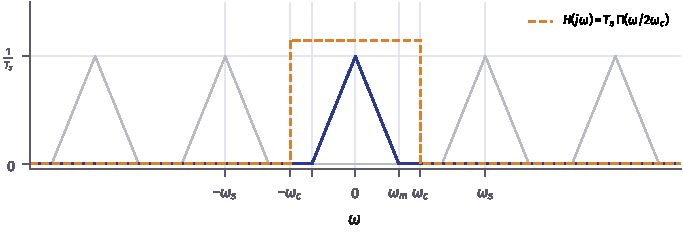
\includegraphics[width=0.72\linewidth]{reconstruccion_ideal}\end{center}
  \begin{definicion}[Filtro paso bajo ideal de reconstrucción]
    \[
      H(j\omega)=T_s\,\rect\Big(\frac{\omega}{2\omega_c}\Big)=\begin{cases}T_s & \abs{\omega}\le\omega_c\\0 & \abs{\omega}>\omega_c\end{cases},\qquad \omega_m<\omega_c<\omega_s-\omega_m
    \]
  \end{definicion}
  \begin{itemize}\small
    \item La ganancia $T_s$ compensa el escalado $1/T_s$ del muestreo: $Y(j\omega)=H(j\omega)X_s(j\omega)=X(j\omega)$.
    \item La elección más habitual es $\omega_c=\omega_s/2$, la única válida cuando el margen es mínimo.
  \end{itemize}
\end{frame}

\begin{frame}{Respuesta al impulso del filtro ideal}
  \[
    h(t)=\frac{1}{2\pi}\int_{-\omega_c}^{\omega_c}T_s\,\e^{j\omega t}\dd\omega
    =\frac{T_s}{\pi t}\sin(\omega_ct)
    =\frac{\omega_cT_s}{\pi}\Sa(\omega_ct)
  \]
  \begin{columns}[c]
    \begin{column}{0.52\textwidth}
      \begin{itemize}\small
        \item Con $\omega_c=\omega_s/2=\pi/T_s$:
        \[h(t)=\sinc\Big(\frac{t}{T_s}\Big)\]
        \item Vale $1$ en $t=0$ y se anula en todos los demás múltiplos de $T_s$.
        \item Es \alert{no causal} y de duración infinita: no se puede construir, solo aproximar.
      \end{itemize}
    \end{column}
    \begin{column}{0.46\textwidth}
      \begin{importante}[Recuerda]
        $\Sa(x)=\dfrac{\sin x}{x}$, \qquad $\sinc(x)=\dfrac{\sin(\pi x)}{\pi x}$\\[1mm]
        $\dfrac{\omega_cT_s}{\pi}\Sa(\omega_ct)=\dfrac{2f_c}{f_s}\sinc(2f_ct)$
      \end{importante}
    \end{column}
  \end{columns}
\end{frame}

\begin{frame}{Fórmula de interpolación}
  Como $x_s(t)=\sum_nx[n]\,\delta(t-nT_s)$, la salida es una suma de respuestas al impulso desplazadas:
  \begin{importante}[Interpolación de Whittaker–Shannon ($\omega_c=\omega_s/2$)]
    \[
      y(t)=\sum_{n=-\infty}^{\infty}x[n]\,h(t-nT_s)=\sum_{n=-\infty}^{\infty}x[n]\,\sinc\Big(\frac{t-nT_s}{T_s}\Big)
    \]
  \end{importante}
  \begin{columns}[c]
    \begin{column}{0.56\textwidth}
      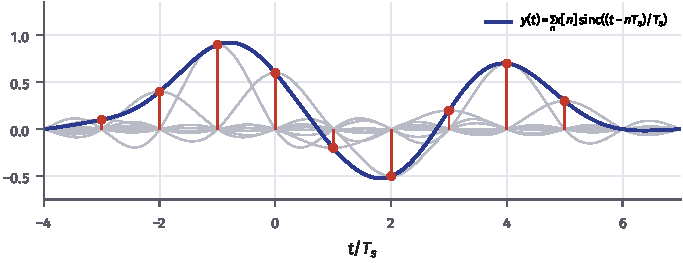
\includegraphics[width=\linewidth]{interpolacion_sinc}
    \end{column}
    \begin{column}{0.42\textwidth}
      \begin{itemize}\small
        \item En $t=nT_s$ solo contribuye la muestra $n$: $y(nT_s)=x[n]$.
        \item Entre muestras, contribuyen \alert{todas}, ponderadas por su distancia.
        \item Si se cumple Nyquist, $y(t)=x(t)$ exactamente.
      \end{itemize}
    \end{column}
  \end{columns}
\end{frame}

\begin{frame}{Ejemplo de reconstrucción ideal}
  \small
  Reconstruir $x(t)=\sin(\omega_0t)$, con $\omega_0=\frac{2\pi}{10}$\,rad/s, a partir de sus muestras con $T_s=4$\,s.
  \begin{itemize}
    \item $\omega_s=\frac{2\pi}{4}>2\omega_0=\frac{4\pi}{10}$: se cumple Nyquist.
    \item Cualquier $\omega_c$ con $\omega_0<\omega_c<\omega_s-\omega_0$, es decir, $\frac{2\pi}{10}<\omega_c<\frac{3\pi}{10}$, reconstruye la señal:
    \[
      y(t)=\sum_nx[n]\,\frac{\omega_cT_s}{\pi}\Sa\big(\omega_c(t-nT_s)\big)
    \]
  \end{itemize}
  \begin{center}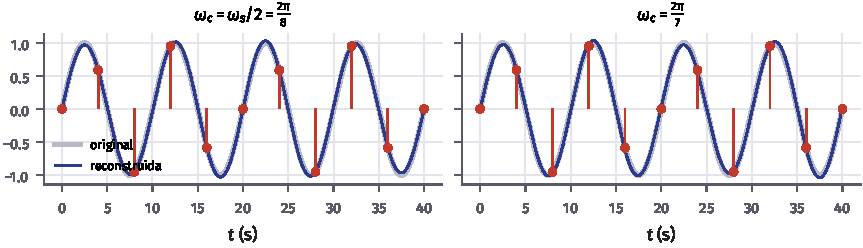
\includegraphics[height=0.36\textheight]{ejemplo_reconstruccion}\end{center}
  \herramienta{html/T2\_Reconstrucción.html}
\end{frame}

\begin{frame}{¿Por qué no basta con el filtro ideal?}
  \begin{itemize}
    \item $h(t)$ es \alert{no causal}: $y(t)$ depende de muestras futuras.
    \item La suma tiene \alert{infinitos términos}, que decaen solo como $1/t$.
    \item Las señales de duración finita \alert{no son de banda limitada}: siempre hay algo de aliasing, aunque sea pequeño.
    \item Un filtro analógico no puede tener un corte abrupto.
  \end{itemize}
  \begin{block}{En la práctica}
    \begin{itemize}\small
      \item Se trunca la suma (fuera de línea, por ejemplo al remuestrear audio o imágenes).
      \item En tiempo real se usan \alert{retenedores}, que interpolan con pocas muestras, seguidos de un filtro analógico de suavizado.
    \end{itemize}
  \end{block}
\end{frame}

\begin{frame}{En código: interpolación con sinc}
  \codigo{reconstruccion_sinc}
  \nota{El error no es exactamente cero porque la suma se trunca a 101 muestras.}
\end{frame}

% =====================================================================
\section{Reconstrucción con retenedores}

\begin{frame}{Reconstrucción como interpolación}
  Cualquier reconstrucción lineal e invariante tiene la forma
  \[
    y(t)=\sum_{n}x[n]\,h(t-nT_s)\qquad\Longleftrightarrow\qquad Y(j\omega)=H(j\omega)\,X_s(j\omega)
  \]
  \begin{itemize}
    \item $h(t)$ es la \alert{función de interpolación}: la contribución de cada muestra según su distancia al instante $t$.
    \item $H(j\omega)$ dice cuánto se atenúan la réplica central y las demás.
  \end{itemize}
  \begin{center}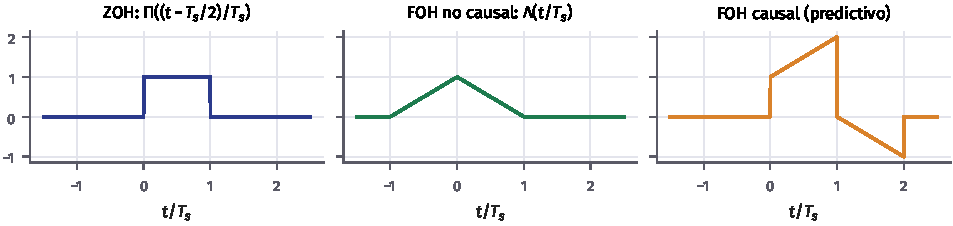
\includegraphics[width=0.9\linewidth]{retenedores_h}\end{center}
\end{frame}

\begin{frame}{Retenedor de orden cero (ZOH)}
  \begin{columns}[c]
    \begin{column}{0.5\textwidth}
      \small
      Mantiene cada muestra hasta la siguiente:
      \[
        h_0(t)=\rect\Big(\frac{t-T_s/2}{T_s}\Big)
      \]
      $y(t)=x[n]$ en $nT_s\le t<(n+1)T_s$.
      \begin{importante}[Respuesta en frecuencia]
        \[
          H_0(j\omega)=T_s\,\e^{-j\omega T_s/2}\,\sinc\Big(\frac{\omega}{\omega_s}\Big)
        \]
      \end{importante}
      \gris{El factor $\e^{-j\omega T_s/2}$ es un retardo de media muestra.}
    \end{column}
    \begin{column}{0.48\textwidth}
      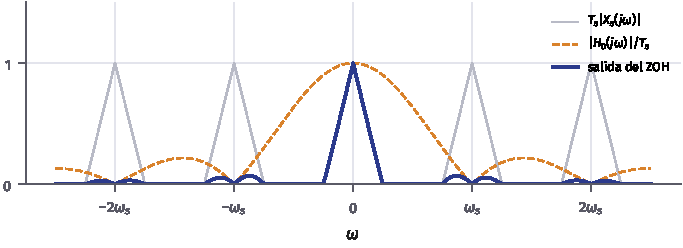
\includegraphics[width=\linewidth]{zoh_espectro}
    \end{column}
  \end{columns}
  \begin{itemize}\small
    \item Es causal y muy sencillo: es lo que hace un conversor D/A.
    \item Atenúa la banda útil: en $\omega_s/2$, $\abs{H_0}/T_s=2/\pi$, unos $-3{,}9$\,dB.
    \item No elimina las réplicas, solo las atenúa: hace falta un \alert{filtro de suavizado} después.
  \end{itemize}
\end{frame}

\begin{frame}{Retenedor de orden uno (FOH)}
  \begin{columns}[T]
    \begin{column}{0.5\textwidth}
      \small
      \alert{No causal}: une las muestras con rectas.
      \[
        h_1(t)=\tri\Big(\frac{t}{T_s}\Big),\qquad H_1(j\omega)=T_s\,\sinc^2\Big(\frac{\omega}{\omega_s}\Big)
      \]
      \begin{itemize}\small
        \item Entre $nT_s$ y $(n+1)T_s$:
        $y(t)=x[n]+\big(x[n+1]-x[n]\big)\frac{t-nT_s}{T_s}$.
        \item Usa la muestra siguiente: retrasándolo $T_s$ se vuelve causal.
        \item Las réplicas caen como $1/\omega^2$.
      \end{itemize}
    \end{column}
    \begin{column}{0.48\textwidth}
      \small
      \alert{Causal (predictivo)}: prolonga la recta de las dos últimas muestras.
      \[
        y(t)=x[n]+\big(x[n]-x[n-1]\big)\frac{t-nT_s}{T_s}
      \]
      $h(t)$: rampa $1+t/T_s$ en $[0,T_s)$ y $1-t/T_s$ en $[T_s,2T_s)$.
      \[H(j\omega)=T_s(1+j\omega T_s)\,\e^{-j\omega T_s}\sinc^2\Big(\frac{\omega}{\omega_s}\Big)\]
    \end{column}
  \end{columns}
\end{frame}

\begin{frame}{Retenedores sobre una misma señal}
  \begin{center}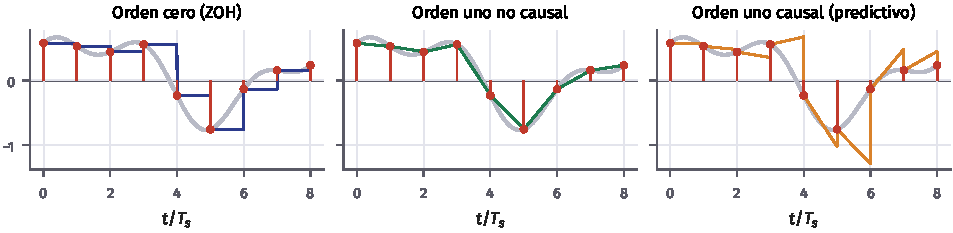
\includegraphics[width=\linewidth]{retenedores_tiempo}\end{center}
  \begin{itemize}\small
    \item El ZOH produce una escalera retrasada media muestra.
    \item El FOH no causal sigue la señal con mucha más precisión, a costa de una muestra de retardo.
    \item El FOH causal no tiene retardo, pero sobrepasa la señal en los cambios de pendiente.
  \end{itemize}
\end{frame}

\begin{frame}{Comparación de los retenedores}
  \begin{columns}[c]
    \begin{column}{0.54\textwidth}
      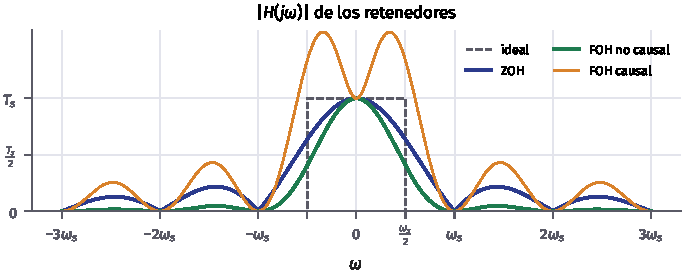
\includegraphics[width=\linewidth]{retenedores_frecuencia}
    \end{column}
    \begin{column}{0.44\textwidth}
      \footnotesize
      \renewcommand{\arraystretch}{1.3}
      \begin{tabular}{@{}lll@{}}
        \toprule
        & $h(t)$ & $\abs{H(j\omega)}/T_s$\\\midrule
        Ideal & $\sinc(t/T_s)$ & $\rect(\omega/\omega_s)$\\
        ZOH & $\rect\big(\frac{t-T_s/2}{T_s}\big)$ & $\abs{\sinc(\omega/\omega_s)}$\\
        FOH & $\tri(t/T_s)$ & $\sinc^2(\omega/\omega_s)$\\\bottomrule
      \end{tabular}
    \end{column}
  \end{columns}
  \begin{itemize}\small
    \item Ningún retenedor reconstruye exactamente: deforman la banda útil y dejan pasar parte de las réplicas.
    \item Cuanto mayor es el orden, mejor atenúan las réplicas, pero necesitan más muestras (y más retardo).
    \item El FOH causal amplifica las altas frecuencias: su salida tiene saltos.
  \end{itemize}
  \herramienta{html/T2\_Retenedores.html}
\end{frame}

\begin{frame}{Conversión D/A en la práctica}
  \begin{center}
    \begin{tikzpicture}[node distance=1.0cm]
      \node (y) {$y[n]$};
      \node[bloque, right=of y] (c) {Compensación\\$1/\sinc$ (digital)};
      \node[bloque, right=of c] (d) {D/A\\(ZOH)};
      \node[bloque, right=of d] (f) {Filtro de\\suavizado};
      \node[right=of f] (o) {$y(t)$};
      \draw[flecha] (y) -- (c); \draw[flecha] (c) -- (d); \draw[flecha] (d) -- (f); \draw[flecha] (f) -- (o);
    \end{tikzpicture}
  \end{center}
  \begin{itemize}
    \item El conversor D/A entrega una señal en escalera: un ZOH.
    \item La caída $\sinc(\omega/\omega_s)$ de la banda útil se puede compensar antes, con un filtro digital.
    \item El filtro analógico de suavizado elimina las réplicas que deja el ZOH.
    \item Con \alert{sobremuestreo} (parte 4), las réplicas se alejan y el filtro analógico puede ser muy sencillo.
  \end{itemize}
\end{frame}

\begin{frame}{En código: retenedores}
  \codigo{retenedores}
  \nota{Con $f_s=10$ muestras por periodo, el error máximo del ZOH es $0{,}59$ y el del FOH, $0{,}05$.}
\end{frame}

% =====================================================================
\section*{Resumen}
\begin{frame}{Conceptos importantes}
  \begin{columns}[T]
    \begin{column}{0.5\textwidth}
      \begin{itemize}
        \item Reconstruir es filtrar: quedarse con la réplica central.
        \item Filtro ideal: $H=T_s\rect(\omega/2\omega_c)$, con $\omega_m<\omega_c<\omega_s-\omega_m$.
        \item Interpolación: $y(t)=\sum x[n]\,\sinc\big(\frac{t-nT_s}{T_s}\big)$.
        \item El filtro ideal no es causal ni realizable.
      \end{itemize}
    \end{column}
    \begin{column}{0.5\textwidth}
      \begin{itemize}
        \item Retenedores: $y(t)=\sum x[n]\,h(t-nT_s)$.
        \item ZOH: $H_0=T_s\e^{-j\omega T_s/2}\sinc(\omega/\omega_s)$.
        \item FOH: $H_1=T_s\sinc^2(\omega/\omega_s)$.
        \item D/A real: ZOH, compensación y filtro de suavizado.
      \end{itemize}
    \end{column}
  \end{columns}
  \bigskip
  \gris{Apuntes del Tema 2, sección 4 · Hoja de ejercicios, ejercicios 7–10.}
\end{frame}

\end{document}
